\newpage
\chapter{ANÁLISIS DEL SISTEMA DE INFORMACIÓN}
	\vspace{2cm}	
	\begin{center}
	{\Large \textbf{FASE DE DESARROLLO} \par}
	\end{center}
	\vspace{5cm}
	
	\begin{center}
	\Huge \textbf{ASI}\par
	\end{center}

%\newpage
%\section{ASI 1: DEFINICIÓN DEL SISTEMA}

%\subsection{Determinación del Alcance del Sistema}



\newpage
\section{ASI 2: ESTABLECIMIENTO DE REQUISITOS}
\subsection{Obtención de los Requisitos del Sistema} 

\subsubsection{Requisitos de interfaces externas}

\paragraph*{Interfaces de usuario}
	
	\newlist{myEnumIU}{enumerate}{4}
	\setlist[myEnumIU,1]{label=\textbf{RIU-\arabic*.}}
	\setlist[myEnumIU,2]{label*=\textbf{\arabic*.}}
	\setlist[myEnumIU,3]{label*=\textbf{\arabic*.}}
	\setlist[myEnumIU,4]{label*=\textbf{\arabic*.}}

	\begin{myEnumIU}
		\item El sistema será accesible desde cualquier dispositivo que cuente con conexión a internet y un navegador web.
		\item El sistema estará disponible en diferentes idiomas.
		\begin{myEnumIU}
			\item Español
			\item Inglés
		\end{myEnumIU}
		\item El sistema deberá ser accesible para todos los usuarios a través de los navegadores más comunes.
		\begin{myEnumIU}
			\item Google Chrome
			\item Mozilla Firefox
			\item Microsoft Edge
		\end{myEnumIU}
		\item El usuario podrá utilizar todas las funcionalidades desarrolladas de la aplicación sin inconvenientes.
		\item El usuario no necesitará de conocimientos tecnológicos avanzados.
	\end{myEnumIU}

\paragraph*{Interfaces hardware}
	
	\newlist{myEnumIH}{enumerate}{4}
	\setlist[myEnumIH,1]{label=\textbf{RIH-\arabic*.}}
	\setlist[myEnumIH,2]{label*=\textbf{\arabic*.}}
	\setlist[myEnumIH,3]{label*=\textbf{\arabic*.}}
	\setlist[myEnumIH,4]{label*=\textbf{\arabic*.}}

	\begin{myEnumIH}
		\item El sistema dispondrá de una base de datos para almacenar la información necesaria.
	\end{myEnumIH}

%\paragraph*{Interfaces software}

\paragraph*{Interfaces de comunicaciones}

	\newlist{myEnumIC}{enumerate}{4}
	\setlist[myEnumIC,1]{label=\textbf{RIC-\arabic*.}}
	\setlist[myEnumIC,2]{label*=\textbf{\arabic*.}}
	\setlist[myEnumIC,3]{label*=\textbf{\arabic*.}}
	\setlist[myEnumIC,4]{label*=\textbf{\arabic*.}}

	\begin{myEnumIC}
		\item El sistema contendrá enlaces a diferentes sitios web.
		\item El sistema mostrará por defecto enlaces a los siguientes sitios web.
		\begin{myEnumIC}
			\item Twitter oficial de la Escuela de Ingeniería Informática
			\item Página web de la Escuela de Ingeniería Informática
			\item Página web de la Universidad de Oviedo
		\end{myEnumIC}
	\end{myEnumIC}



\subsubsection{Requisitos funcionales}

\newlist{myEnumerate}{enumerate}{9}
\setlist[myEnumerate,1]{label=\textbf{RF-\arabic*.}}
\setlist[myEnumerate,2]{label*=\textbf{\arabic*.}}
\setlist[myEnumerate,3]{label*=\textbf{\arabic*.}}
\setlist[myEnumerate,4]{label*=\textbf{\arabic*.}}
\setlist[myEnumerate,5]{label*=\textbf{\arabic*.}}
\setlist[myEnumerate,6]{label*=\textbf{\arabic*.}}
\setlist[myEnumerate,7]{label*=\textbf{\arabic*.}}
\setlist[myEnumerate,8]{label*=\textbf{\arabic*.}}
\setlist[myEnumerate,9]{label*=\textbf{\arabic*.}}

\begin{myEnumerate}
\item
\end{myEnumerate}


\subsubsection{Requisitos de rendimiento}
\subsubsection{Requisitos lógicos de BD}
\subsubsection{Requisitos de desarrollo}
\subsubsection{Restricciones de diseño}
\subsubsection{Atributos del sistema}


\subsection{Identificación de Actores del Sistema} 
\subsubsection{Usuario administrador}
Actor que interactúa con el sistema. Es responsable de gestionar el sistema y su mantenimiento. Es el único actor con acceso a la base de datos del sistema y capacidad de modificarla. Debe tener amplios conocimientos sobre el sistema.
\subsubsection{Usuario estándar}
Actor que interactúa con el sistema. Tiene acceso de lectura a toda la aplicación web, exceptuando la parte dedicada al mantenimiento. Solo debe tener un conocimiento básico para navegar por internet.

\subsection{Especificación de Casos de Uso}

\textcolor[rgb]{0.65,0.16,0}{Ejemplo de tabla para especificación de casos de uso}

\begin{table}[htbp]
  \centering
  \caption{Especificación Caso de Uso 1}
    \begin{tabular}{p{20.855em}r}
\cmidrule{1-1}    \rowcolor[rgb]{ .949,  .949,  .949} \multicolumn{1}{p{20.855em}}{\textbf{Nombre del caso de uso}} & \multicolumn{1}{r}{\cellcolor[rgb]{ 1,  1,  1}} \\
\cmidrule{1-1}    \multicolumn{1}{p{20.855em}}{Registro} & \multicolumn{1}{r}{} \\
    \midrule
    \rowcolor[rgb]{ .949,  .949,  .949} \multicolumn{2}{p{31.64em}}{\textbf{Descripción}} \\
    \midrule
    \multicolumn{2}{p{31.64em}}{Un usuario no registrado debe poder registrarse en el sistema mediante su cuenta de Google, lo que hará que automáticamente se inicie sesión en la aplicación.} \\
    \bottomrule
    \end{tabular}%
  \label{espec_caso_uso_1}%
  \vspace{-4mm}
\end{table}%



%\newpage
%\section{ASI 3: IDENTIFICACIÓN DE SUBSISTEMAS DE ANÁLISIS}
%
%\subsection{Descripción de los Subsistemas} 
%%A continuación se describen los subsistemas identificados en el análisis
%%\subsubsection{Vistas}
%%
%%\subsubsection{Modelos}
%%
%%\subsubsection{Bases de datos}
%%
%%\subsubsection{Servidor}
%
%
%\subsection{Descripción de los Interfaces entre Subsistemas}



\newpage
\section{ASI 4: ANÁLISIS DE LOS CASOS DE USO}
\subsection{Caso de Uso 1} 

\begin{table}[H]
  \centering
  \vspace{-5mm}
  \caption{Análisis del Caso de Uso 1}
    \begin{tabular}{p{7.5em}p{24.145em}}
    \toprule
    \rowcolor[rgb]{ .871,  .918,  .965} \multicolumn{2}{p{31.645em}}{\textbf{Consultar periodos (museo)}} \\
    \midrule
    \rowcolor[rgb]{ .906,  .902,  .902} \textbf{Precondiciones} & \cellcolor[rgb]{ 1,  1,  1}- \\
    \midrule
    \rowcolor[rgb]{ .906,  .902,  .902} \textbf{Postcondiciones} & \cellcolor[rgb]{ 1,  1,  1}- \\
    \midrule
    \rowcolor[rgb]{ .906,  .902,  .902} \textbf{Actores} & \cellcolor[rgb]{ 1,  1,  1}Usuario estándar \\
    \midrule
    \rowcolor[rgb]{ .906,  .902,  .902} \textbf{Descripción} & \cellcolor[rgb]{ 1,  1,  1}El usuario accederá a la vista principal del museo y podrá visualizar los periodos existentes. Podrá acceder a los periodos. Podrá acceder a los componentes de los periodos. Podrá realizar una búsqueda.\\
    \midrule
    \rowcolor[rgb]{ .906,  .902,  .902} \textbf{Escenarios          Secundarios} & \cellcolor[rgb]{ 1,  1,  1}  \\
    \bottomrule
    \end{tabular}%
\end{table}%
 
\subsection{Caso de Uso 2}
\begin{table}[H]
  \centering
  \vspace{-5mm}
  \caption{Análisis del Caso de Uso 2}
    \begin{tabular}{p{7.5em}p{24.145em}}
    \toprule
    \rowcolor[rgb]{ .871,  .918,  .965} \multicolumn{2}{p{31.645em}}{\textbf{Consultar componentes (museo)}} \\
    \midrule
    \rowcolor[rgb]{ .906,  .902,  .902} \textbf{Precondiciones} & \cellcolor[rgb]{ 1,  1,  1}- \\
    \midrule
    \rowcolor[rgb]{ .906,  .902,  .902} \textbf{Postcondiciones} & \cellcolor[rgb]{ 1,  1,  1}- \\
    \midrule
    \rowcolor[rgb]{ .906,  .902,  .902} \textbf{Actores} & \cellcolor[rgb]{ 1,  1,  1}Usuario estándar \\
    \midrule
    \rowcolor[rgb]{ .906,  .902,  .902} \textbf{Descripción} & \cellcolor[rgb]{ 1,  1,  1}El usuario accederá a la vista de un periodo y podrá visualizar los componentes pertenecientes al mismo. Podrá acceder a otros periodos. Podrá acceder a los otros componentes de ese periodo. \\
    \midrule
    \rowcolor[rgb]{ .906,  .902,  .902} \textbf{Escenarios          Secundarios} & \cellcolor[rgb]{ 1,  1,  1}  \\
    \bottomrule
    \end{tabular}%
\end{table}%
 
\subsection{Caso de Uso 3}
\begin{table}[H]
  \centering
  \vspace{-5mm}
  \caption{Análisis del Caso de Uso 3}
    \begin{tabular}{p{7.5em}p{24.145em}}
    \toprule
    \rowcolor[rgb]{ .871,  .918,  .965} \multicolumn{2}{p{31.645em}}{\textbf{Iniciar sesión}} \\
    \midrule
    \rowcolor[rgb]{ .906,  .902,  .902} \textbf{Precondiciones} & \cellcolor[rgb]{ 1,  1,  1}El usuario no debe haber iniciado sesión. \\
    \midrule
    \rowcolor[rgb]{ .906,  .902,  .902} \textbf{Postcondiciones} & \cellcolor[rgb]{ 1,  1,  1}- \\
    \midrule
    \rowcolor[rgb]{ .906,  .902,  .902} \textbf{Actores} & \cellcolor[rgb]{ 1,  1,  1}Usuario \\
    \midrule
    \rowcolor[rgb]{ .906,  .902,  .902} \textbf{Descripción} & \cellcolor[rgb]{ 1,  1,  1}El usuario accederá a la página principal de la aplicación de administración e introducirá su email y contraseña para iniciar sesión en el sistema. \\
    \midrule
    \rowcolor[rgb]{ .906,  .902,  .902} \textbf{Escenarios          Secundarios} & \cellcolor[rgb]{ 1,  1,  1} Los datos introducidos no se corresponden con los datos de un usuario con permiso de administrador. Se muestra un error y de nuevo se solicita iniciar sesión. \\
    \bottomrule
    \end{tabular}%
\end{table}%
 
\subsection{Caso de Uso 4}
\begin{table}[H]
  \centering
  \vspace{-5mm}
  \caption{Análisis del Caso de Uso 4}
    \begin{tabular}{p{7.5em}p{24.145em}}
    \toprule
    \rowcolor[rgb]{ .871,  .918,  .965} \multicolumn{2}{p{31.645em}}{\textbf{Consultar periodos (administración)}} \\
    \midrule
    \rowcolor[rgb]{ .906,  .902,  .902} \textbf{Precondiciones} & \cellcolor[rgb]{ 1,  1,  1}El usuario debe haber iniciado sesión. \\
    \midrule
    \rowcolor[rgb]{ .906,  .902,  .902} \textbf{Postcondiciones} & \cellcolor[rgb]{ 1,  1,  1}- \\
    \midrule
    \rowcolor[rgb]{ .906,  .902,  .902} \textbf{Actores} & \cellcolor[rgb]{ 1,  1,  1}Usuario administrador \\
    \midrule
    \rowcolor[rgb]{ .906,  .902,  .902} \textbf{Descripción} & \cellcolor[rgb]{ 1,  1,  1}El usuario accederá al listado de periodos. Podrá acceder a cada uno de ellos. \\
    \midrule
    \rowcolor[rgb]{ .906,  .902,  .902} \textbf{Escenarios          Secundarios} & \cellcolor[rgb]{ 1,  1,  1}Aún no existe ningún periodo en el sistema. Se muestra una tabla vacía. \\
    \bottomrule
    \end{tabular}%
\end{table}
 
\subsection{Caso de Uso 5}
\begin{table}[H]
  \centering
  \vspace{-5mm}
  \caption{Análisis del Caso de Uso 5}
    \begin{tabular}{p{7.5em}p{24.145em}}
    \toprule
    \rowcolor[rgb]{ .871,  .918,  .965} \multicolumn{2}{p{31.645em}}{\textbf{Añadir periodo}} \\
    \midrule
    \rowcolor[rgb]{ .906,  .902,  .902} \textbf{Precondiciones} & \cellcolor[rgb]{ 1,  1,  1}El usuario debe haber iniciado sesión. \\
    \midrule
    \rowcolor[rgb]{ .906,  .902,  .902} \textbf{Postcondiciones} & \cellcolor[rgb]{ 1,  1,  1}El periodo añadido se guardará en la base de datos. \\
    \midrule
    \rowcolor[rgb]{ .906,  .902,  .902} \textbf{Actores} & \cellcolor[rgb]{ 1,  1,  1}Usuario administrador \\
    \midrule
    \rowcolor[rgb]{ .906,  .902,  .902} \textbf{Descripción} & \cellcolor[rgb]{ 1,  1,  1}El usuario accede al formulario para añadir un periodo. Rellena los campos necesarios. Pulsa el botón de guardar. \\
    \midrule
    \rowcolor[rgb]{ .906,  .902,  .902} \textbf{Escenarios          Secundarios} & \cellcolor[rgb]{ 1,  1,  1}- Se pulsa el botón cancelar. El formulario se restablece.\par - Se intenta acceder a otra página de la aplicación sin haber guardado los cambios. Se avisa de la situación y se pide una confirmación para continuar.\par - No se puede añadir el periodo. Se mostrará un error avisando de la situación. \\
    \bottomrule
    \end{tabular}%
\end{table}%
 
\subsection{Caso de Uso 6}
\begin{table}[H]
  \centering
  \vspace{-5mm}
  \caption{Análisis del Caso de Uso 6}
    \begin{tabular}{p{7.5em}p{24.145em}}
    \toprule
    \rowcolor[rgb]{ .871,  .918,  .965} \multicolumn{2}{p{31.645em}}{\textbf{Modificar periodo}} \\
    \midrule
    \rowcolor[rgb]{ .906,  .902,  .902} \textbf{Precondiciones} & \cellcolor[rgb]{ 1,  1,  1}El usuario debe haber iniciado sesión. Debe existir al menos un periodo. \\
    \midrule
    \rowcolor[rgb]{ .906,  .902,  .902} \textbf{Postcondiciones} & \cellcolor[rgb]{ 1,  1,  1}Los cambios realizados al periodo se guardarán en la base de datos. \\
    \midrule
    \rowcolor[rgb]{ .906,  .902,  .902} \textbf{Actores} & \cellcolor[rgb]{ 1,  1,  1}Usuario administrador \\
    \midrule
    \rowcolor[rgb]{ .906,  .902,  .902} \textbf{Descripción} & \cellcolor[rgb]{ 1,  1,  1}El usuario accede al periodo deseado y selecciona la opción de editar. Se mostrará el formulario correspondiente. Se realizan los cambios en el formulario. Pulsa el botón de guardar. \\
    \midrule
    \rowcolor[rgb]{ .906,  .902,  .902} \textbf{Escenarios          Secundarios} & \cellcolor[rgb]{ 1,  1,  1}- Se pulsa el botón cancelar. El formulario se restablece.\par - Se intenta acceder a otra página de la aplicación sin haber guardado los cambios. Se avisa de la situación y se pide una confirmación para continuar.\par - No se puede modificar el periodo. Se mostrará un error avisando de la situación. \\
    \bottomrule
    \end{tabular}%
\end{table}%
 
\subsection{Caso de Uso 7}
\begin{table}[H]
  \centering
  \vspace{-5mm}
  \caption{Análisis del Caso de Uso 7}
    \begin{tabular}{p{7.5em}p{24.145em}}
    \toprule
    \rowcolor[rgb]{ .871,  .918,  .965} \multicolumn{2}{p{31.645em}}{\textbf{Eliminar periodo}} \\
    \midrule
    \rowcolor[rgb]{ .906,  .902,  .902} \textbf{Precondiciones} & \cellcolor[rgb]{ 1,  1,  1}El usuario debe haber iniciado sesión. Debe existir al menos un periodo. \\
    \midrule
    \rowcolor[rgb]{ .906,  .902,  .902} \textbf{Postcondiciones} & \cellcolor[rgb]{ 1,  1,  1}El periodo eliminado y los componentes que pertenecen al mismo se borrarán de la base de datos y dejarán de mostrarse en la aplicación. \\
    \midrule
    \rowcolor[rgb]{ .906,  .902,  .902} \textbf{Actores} & \cellcolor[rgb]{ 1,  1,  1}Usuario administrador \\
    \midrule
    \rowcolor[rgb]{ .906,  .902,  .902} \textbf{Descripción} & \cellcolor[rgb]{ 1,  1,  1}El usuario accede al periodo deseado y selecciona la opción de eliminar. Se pide confirmación para eliminarlo. Se acepta esta confirmación. \\
    \midrule
    \rowcolor[rgb]{ .906,  .902,  .902} \textbf{Escenarios          Secundarios} & \cellcolor[rgb]{ 1,  1,  1}- No se acepta la confirmación para eliminarlo. El periodo y sus componentes permanecen en la base de datos.\par - No se puede eliminar el periodo. Se mostrará un error avisando de la situación. \\
    \bottomrule
    \end{tabular}%
\end{table}%
 
\subsection{Caso de Uso 8}
\begin{table}[H]
  \centering
  \vspace{-5mm}
  \caption{Análisis del Caso de Uso 8}
    \begin{tabular}{p{7.5em}p{24.145em}}
    \toprule
    \rowcolor[rgb]{ .871,  .918,  .965} \multicolumn{2}{p{31.645em}}{\textbf{Consultar componentes (administración)}} \\
    \midrule
    \rowcolor[rgb]{ .906,  .902,  .902} \textbf{Precondiciones} & \cellcolor[rgb]{ 1,  1,  1}El usuario debe haber iniciado sesión. Debe existir al menos un periodo. \\
    \midrule
    \rowcolor[rgb]{ .906,  .902,  .902} \textbf{Postcondiciones} & \cellcolor[rgb]{ 1,  1,  1}- \\
    \midrule
    \rowcolor[rgb]{ .906,  .902,  .902} \textbf{Actores} & \cellcolor[rgb]{ 1,  1,  1}Usuario administrador \\
    \midrule
    \rowcolor[rgb]{ .906,  .902,  .902} \textbf{Descripción} & \cellcolor[rgb]{ 1,  1,  1}El usuario accederá a un periodo existente y visualizará los componentes pertenecientes a este. Podrá acceder a cada uno de ellos. \\
    \midrule
    \rowcolor[rgb]{ .906,  .902,  .902} \textbf{Escenarios          Secundarios} & \cellcolor[rgb]{ 1,  1,  1}Aún no existen componentes para el periodo que se consulta. Se mostrará una tabla vacía. \\
    \bottomrule
    \end{tabular}%
\end{table}%
 
\subsection{Caso de Uso 9}
\begin{table}[H]
  \centering
  \vspace{-5mm}
  \caption{Análisis del Caso de Uso 9}
    \begin{tabular}{p{7.5em}p{24.145em}}
    \toprule
    \rowcolor[rgb]{ .871,  .918,  .965} \multicolumn{2}{p{31.645em}}{\textbf{Añadir componente}} \\
    \midrule
    \rowcolor[rgb]{ .906,  .902,  .902} \textbf{Precondiciones} & \cellcolor[rgb]{ 1,  1,  1}El usuario debe haber iniciado sesión. Debe existir al menos un periodo. \\
    \midrule
    \rowcolor[rgb]{ .906,  .902,  .902} \textbf{Postcondiciones} & \cellcolor[rgb]{ 1,  1,  1}El componente añadido se guardará en la base de datos y se asociará al periodo correspondiente. \\
    \midrule
    \rowcolor[rgb]{ .906,  .902,  .902} \textbf{Actores} & \cellcolor[rgb]{ 1,  1,  1}Usuario administrador \\
    \midrule
    \rowcolor[rgb]{ .906,  .902,  .902} \textbf{Descripción} & \cellcolor[rgb]{ 1,  1,  1}El usuario accede al formulario para añadir un componente. Rellena los campos necesarios. Pulsa el botón de guardar. \\
    \midrule
    \rowcolor[rgb]{ .906,  .902,  .902} \textbf{Escenarios          Secundarios} & \cellcolor[rgb]{ 1,  1,  1}- Se pulsa el botón cancelar. El formulario se restablece.\par - Se intenta acceder a otra página de la aplicación sin haber guardado los cambios. Se avisa de la situación y se pide una confirmación para continuar.\par - No se puede añadir el componente. Se mostrará un error avisando de la situación.  \\
    \bottomrule
    \end{tabular}%
\end{table}%
 
\subsection{Caso de Uso 10}
\begin{table}[H]
  \centering
  \vspace{-5mm}
  \caption{Análisis del Caso de Uso 10}
    \begin{tabular}{p{7.5em}p{24.145em}}
    \toprule
    \rowcolor[rgb]{ .871,  .918,  .965} \multicolumn{2}{p{31.645em}}{\textbf{Modificar componente}} \\
    \midrule
    \rowcolor[rgb]{ .906,  .902,  .902} \textbf{Precondiciones} & \cellcolor[rgb]{ 1,  1,  1}El usuario debe haber iniciado sesión. Debe existir al menos un componente. \\
    \midrule
    \rowcolor[rgb]{ .906,  .902,  .902} \textbf{Postcondiciones} & \cellcolor[rgb]{ 1,  1,  1}Los cambios realizados en el componente se guardarán en la base de datos. \\
    \midrule
    \rowcolor[rgb]{ .906,  .902,  .902} \textbf{Actores} & \cellcolor[rgb]{ 1,  1,  1}Usuario administrador \\
    \midrule
    \rowcolor[rgb]{ .906,  .902,  .902} \textbf{Descripción} & \cellcolor[rgb]{ 1,  1,  1}El usuario accede al componente deseado y selecciona la opción de editar. Se mostrará el formulario correspondiente. Se realizan los cambios en el formulario. Pulsa el botón de guardar. \\
    \midrule
    \rowcolor[rgb]{ .906,  .902,  .902} \textbf{Escenarios          Secundarios} & \cellcolor[rgb]{ 1,  1,  1}- Se pulsa el botón cancelar. El formulario se restablece.\par - Se intenta acceder a otra página de la aplicación sin haber guardado los cambios. Se avisa de la situación y se pide una confirmación para continuar.\par - No se puede modificar el componente. Se mostrará un error avisando de la situación.  \\
    \bottomrule
    \end{tabular}%
\end{table}
 
\subsection{Caso de Uso 11}
\begin{table}[H]
  \centering
  \vspace{-5mm}
  \caption{Análisis del Caso de Uso 11}
    \begin{tabular}{p{7.5em}p{24.145em}}
    \toprule
    \rowcolor[rgb]{ .871,  .918,  .965} \multicolumn{2}{p{31.645em}}{\textbf{Eliminar componente}} \\
    \midrule
    \rowcolor[rgb]{ .906,  .902,  .902} \textbf{Precondiciones} & \cellcolor[rgb]{ 1,  1,  1}El usuario debe haber iniciado sesión. Debe existir al menos un componente. \\
    \midrule
    \rowcolor[rgb]{ .906,  .902,  .902} \textbf{Postcondiciones} & \cellcolor[rgb]{ 1,  1,  1}El componente eliminado  se borrará de la base de datos y dejará de mostrarse en la aplicación. \\
    \midrule
    \rowcolor[rgb]{ .906,  .902,  .902} \textbf{Actores} & \cellcolor[rgb]{ 1,  1,  1}Usuario administrador \\
    \midrule
    \rowcolor[rgb]{ .906,  .902,  .902} \textbf{Descripción} & \cellcolor[rgb]{ 1,  1,  1}El usuario accede al componente deseado y selecciona la opción de eliminar. Se pide confirmación para eliminarlo. Se acepta esta confirmación.  \\
    \midrule
    \rowcolor[rgb]{ .906,  .902,  .902} \textbf{Escenarios          Secundarios} & \cellcolor[rgb]{ 1,  1,  1}- No se acepta la confirmación para eliminarlo. El componente permanece en la base de datos.\par - No se puede eliminar el componente. Se mostrará un error avisando de la situación.  \\
    \bottomrule
    \end{tabular}%
\end{table}%


\newpage
\section{ASI 5: ANÁLISIS DE CLASES}

\subsection{Diagrama de Clases} 

\subsection{Descripción de las Clases}


\newpage
\section{ASI 8: DEFINICIÓN DE INTERFACES DE USUARIO}

%\subsection{Descripción de la Interfaz} 

\subsection{Definición del aspecto de la interfaz}

\subsubsection{Museo}
A continuación se presentan los prototipos de interfaces diseñados para la página web del museo. Todas ellas tienen en común la barra de navegación, que contiene el logo de la EII, un enlace a la vista general del museo y un selector de idioma.
\paragraph*{Inicio}
En la página de inicio del museo se muestra un mensaje de bienvenida y un botón que conduce a la vista general del museo.
\begin{figure}[H]
\centering
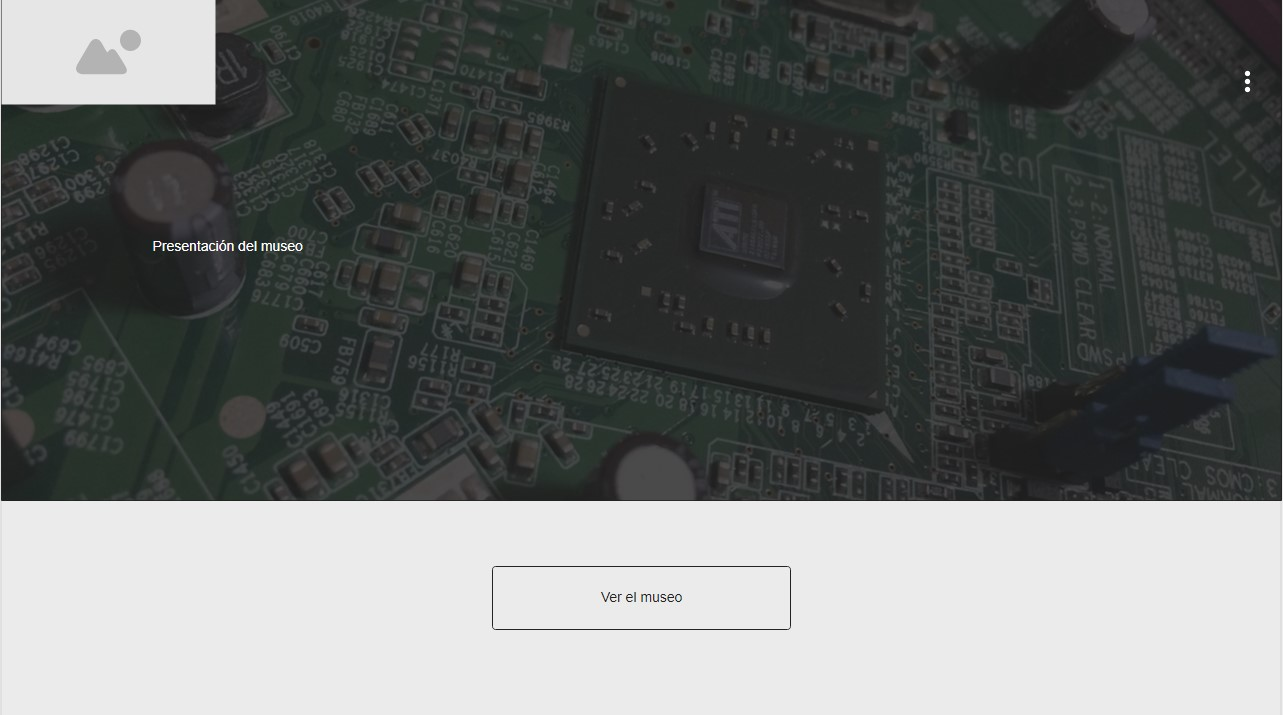
\includegraphics[scale=0.45]{homeIU}
\caption{Prototipo: Página de inicio}
\end{figure}
\paragraph*{Vista general del museo}
En la vista general del museo encontramos un menú lateral con filtros de búsqueda, y una sección principal que contiene una línea temporal con los periodos en los que se divide la historia de las CPUs.
\begin{figure}[H]
\centering
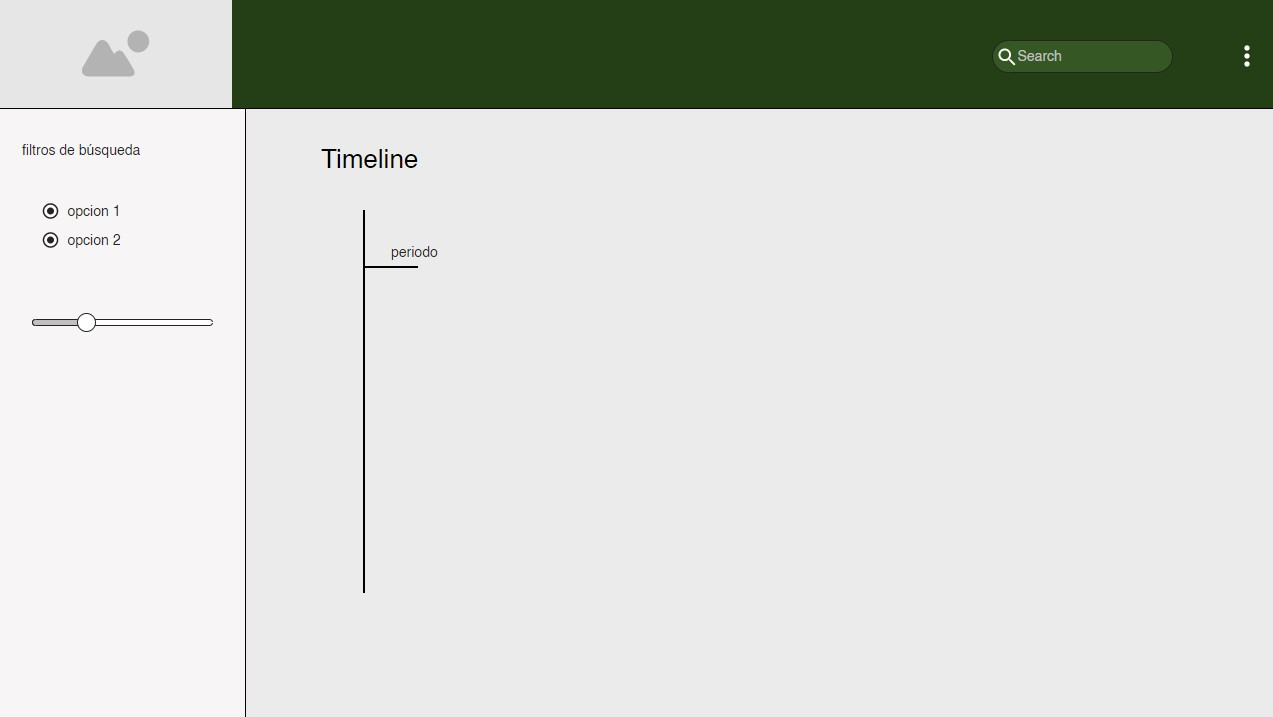
\includegraphics[scale=0.45]{museoIU}
\caption{Prototipo: Página de la vista general del museo}
\end{figure}
\paragraph*{Detalles del periodo}
En esta página hay un menú para volver a la vista general, y se muestran todos los detalles de un periodo (nombre, características, sistemas famosos de dicho periodo, etc.) y los componentes que pertenecen al mismo. 
\begin{figure}[H]
\centering
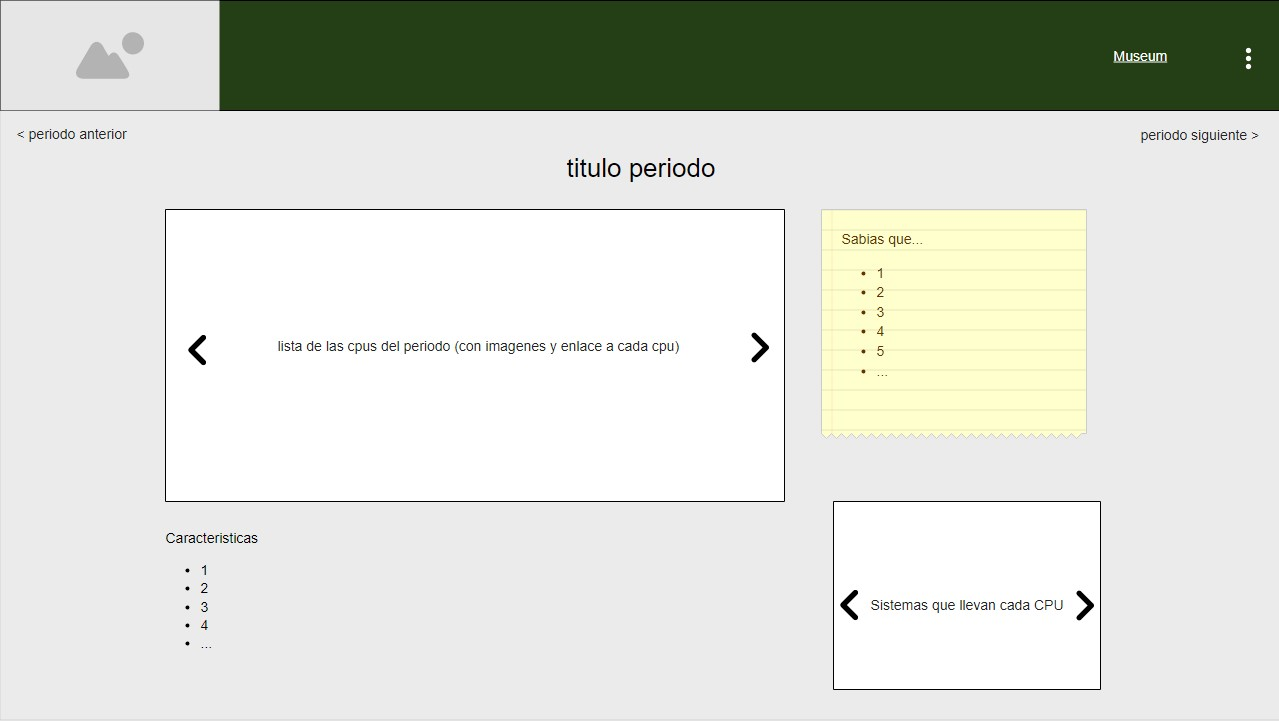
\includegraphics[scale=0.45]{periodoIU}
\caption{Prototipo: Página de detalles del periodo (museo)}
\end{figure}
\paragraph*{Detalles del componente}
En esta página se muestra una galería de fotos del componente, la descripción del mismo, y un listado de características. En el menú de esta página hay un listado de componentes pertenecientes al mismo periodo.
\begin{figure}[H]
\centering
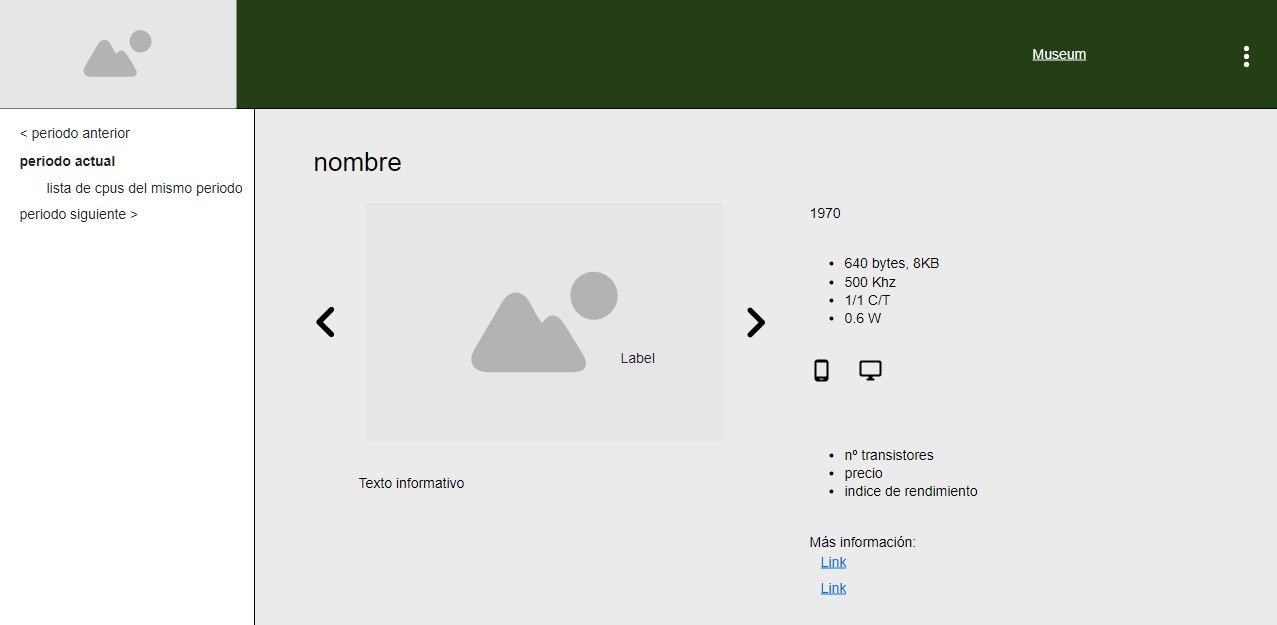
\includegraphics[scale=0.45]{piezaIU}
\caption{Prototipo: Página de detalles del componente (museo)}
\end{figure}

\subsubsection{Administración del museo}
A continuación, se muestran los prototipos inciales para la aplicación de administración del museo. En todas ellas, salvo en la de inicio de sesión, hay un menú lateral de navegación. 
\paragraph*{Iniciar sesión}
En esta página el administrador del sistema deberá introducir su usuario y contraseña para acceder al mismo.
\begin{figure}[H]
\centering
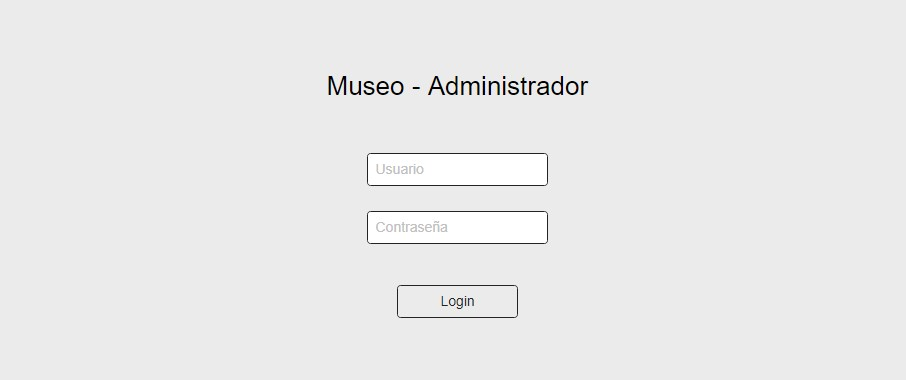
\includegraphics[scale=0.55]{loginIU}
\caption{Prototipo: Página de inicio de sesión}
\end{figure}
\paragraph*{Listado de periodos}
En esta página se muestra un listado de los periodos existentes, con las opciones de acceder a cada uno, editarlo o eliminarlo.
\begin{figure}[H]
\centering
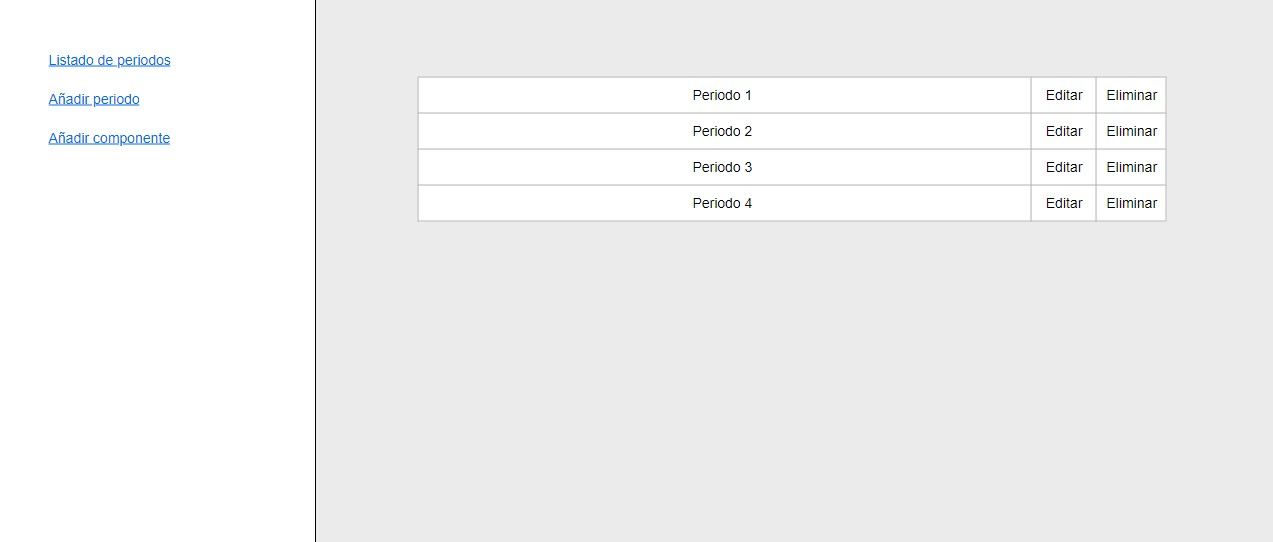
\includegraphics[scale=0.45]{listadoPeriodosIU}
\caption{Prototipo: Página de listado de periodos}
\end{figure}
\paragraph*{Periodo}
Esta página contiene los detalles de un periodo así como un listado de los componentes pertenecientes al mismo, ofreciendo la opción de acceder a ellos, editarlos o eliminarlos.
\begin{figure}[H]
\centering
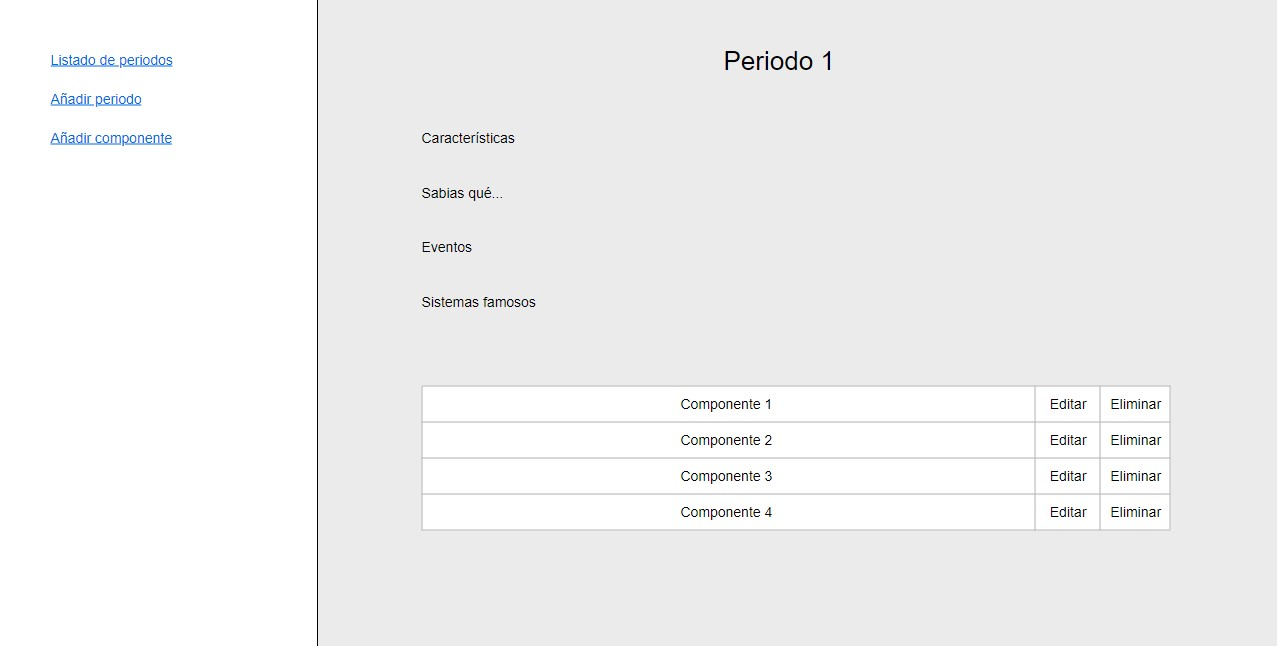
\includegraphics[scale=0.45]{periodoIU2}
\caption{Prototipo: Página de detalles de un periodo (admimnistración)}
\end{figure}
\paragraph*{Componente}
En esta página se muestran los detalles correspondientes al componente.
\begin{figure}[H]
\centering
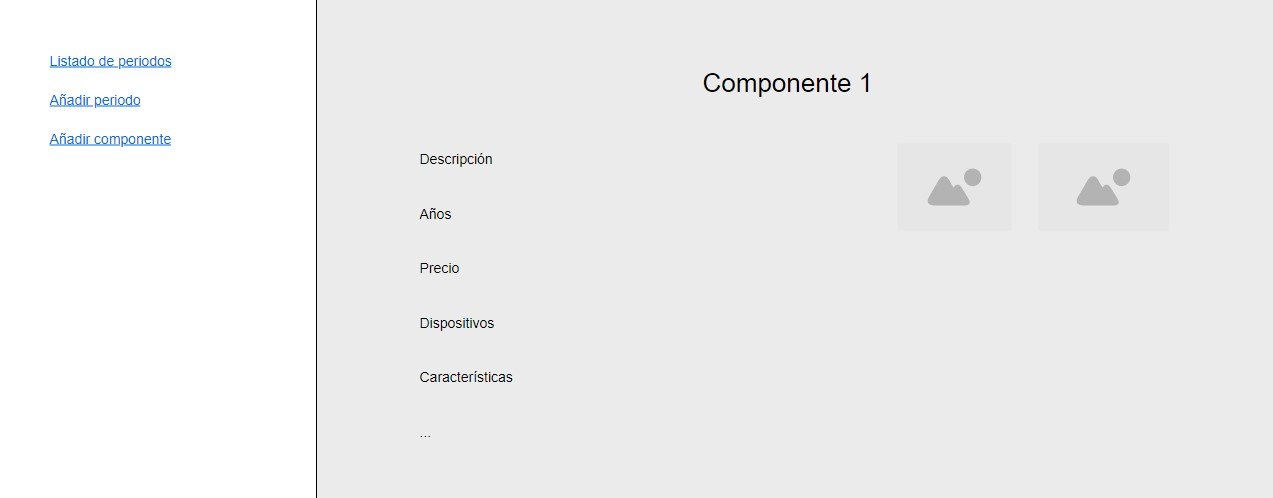
\includegraphics[scale=0.45]{compIU}
\caption{Prototipo: Página de detalles de un componente (admimnistración)}
\end{figure}
\paragraph*{Añadir/editar periodo}
Los formularios para añadir o editar un periodo son idénticos, con la única diferencia de que el formulario para editar ya tiene los campos completados con los valores existentes del periodo, por tanto solo se muestra una captura representando ambos.
\begin{figure}[H]
\centering
\includegraphics[scale=0.45]{añadirPeriodoIU}
\caption{Prototipo: Formulario para añadir o editar un periodo}
\end{figure}
\paragraph*{Añadir/editar componente}
Con los formularios para añadir o editar un componente ocurre igual que con los del periodo ya mencionados.
\begin{figure}[H]
\centering
\includegraphics[scale=0.45]{añadirCompIU}
\caption{Prototipo: Formulario para añadir o editar un componente}
\end{figure}



%\subsection{Descripción del Comportamiento de la Interfaz} 

\subsection{Diagrama de Navegabilidad}
A continuación se presentan dos diagramas de navegabilidad, correspondientes a las dos aplicaciones web que constituyen el sistema.
\subsubsection{Museo}
\begin{figure}[H]
\centering
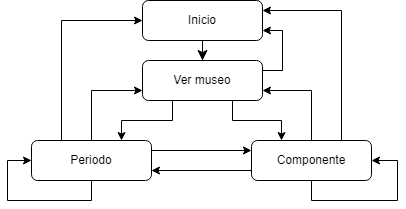
\includegraphics[scale=0.7]{nav-museo}
\caption{Diagrama de navegabilidad del museo}
\end{figure}

\subsubsection{Administración del museo}
\begin{figure}[H]
\centering
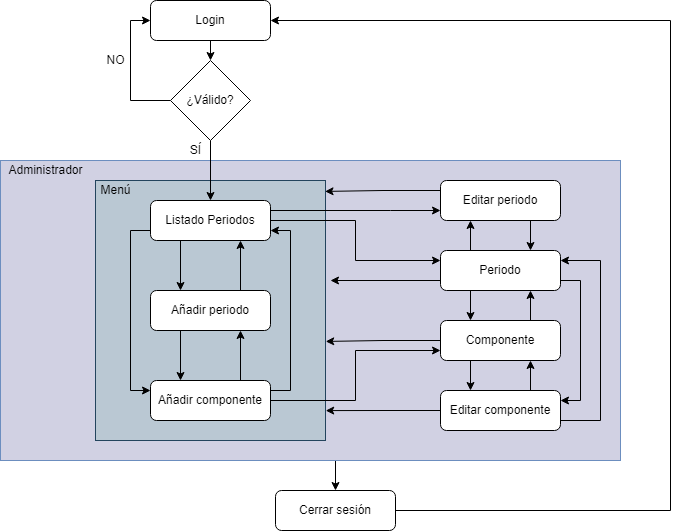
\includegraphics[scale=0.7]{nav-admin}
\caption{Diagrama de navegabilidad de la administración del museo}
\end{figure}

\newpage
\section{ASI 10: ESPECIFICACIÓN DEL PLAN DE PRUEBAS}
